%%%%%%%%%%%%%%%%%%%%%%%%%%%%%%%%%%%%%%%%%%%%%%%%%%%%%%%%%%%%%%%%%%%
%TO AVOID FORMATTING ISSUES, COMPILE THIS ONLY AT WWW.OVERLEAF.COM%
%%%%%%%%%%%%%%%%%%%%%%%%%%%%%%%%%%%%%%%%%%%%%%%%%%%%%%%%%%%%%%%%%%%
%AUTHOR: 
%CLASS:  
%%%%%%%%%%%%%%%%%%%%%%%%%%%%%%%%%%%%%%%%%%%%%%%%%%%%%%%%%%%%%%%%%%%
\documentclass[a4paper,12pt]{article}
\usepackage{graphicx}
\usepackage{listings}
\newenvironment{codefont}{\fontfamily{pcr}\selectfont}{\par}

\title{
	\normalfont \normalsize 
	\textsc{Pimpri Chinchwad College of Engineering \\ 
		Computer Laboratory - III} \\
	[10pt] 
	\rule{\linewidth}{0.5pt} \\[6pt] 
	\huge Assignment No - 2 \\
	\rule{\linewidth}{2pt}  \\[10pt]
}
\author{}
\date{\normalsize}


\begin{document}
\maketitle

%%%%%%%%%%%%%%%%%%%%%%%
% FOR A NUMBERED LIST
% \begin{enumerate}
% \item Your_Item
% \end{enumerate}
%%%%%%%%%%%%%%%%%%%%%%%
% FOR A BULLETED LIST
% \begin{itemize}
% \item Your_Item
% \end{itemize}
%%%%%%%%%%%%%%%%%%%%%%%
% TO IMPORT AN IMAGE
% \includegraphics[width=\textwidth]{name_of_file}
% \textwidth makes the picture the width of the paragraphs
%%%%%%%%%%%%%%%%%%%%%%%%%%%%%%
% TO CREATE A FIGURE WITH A NUMBER AND CAPTION
% \begin{figure}
% \includegraphics[width=\textwidth]{image}
% \caption{Your Caption Goes Here}
% \label{your_label}
% \end{figure}
% REFER TO YOUR FIGURE LATER WITH
% \ref{your_label}
% LABELS NEED TO BE ONE WORD
%%%%%%%%%%%%%%%%%%%%%%%%%%%%%
% TO ADD CODE
% \begin{codefont}
% Some code in "courier" font
%\end{codefont}
%%%%%%%%%%%%%%%%%%%%%%%%%%%%%
\section{Aim}
	\paragraph{} Take a message as an input from user and calculate hash value using SHA algorithm. Develop program in C++/Python/Java.
	
\section{Objective}
	\begin{itemize}
		\item To understand SHA-1 message digest.
		\item To verify data integrity using SHA-1 equivalent hash. 
	\end{itemize}
	
\section{Software Requirements}
	\begin{itemize}
		\item	Operating System : Windows 10, Ubuntu
		\item	Java
		 
	\end{itemize}
	
\section{Mathematical Model}
\paragraph{} 
S 	= {s, e, x, y, Fme, DD, NDD}  											\\\\
S   =   Initial State  														\\
E 	=   End State  															\\
X	= Input Value															\\
X=\{x1\} 																\\
where,  x1= Message from user
\\																\\
Y	= Output																\\
Y=\{y1\}																	\\
y1=\{"Message digest\}									\\
Fme 	= 	Main function 													\\
Fme=\{f1\}\\f1="SHA1 Algorithm to calculate Digest of the Plaintext".		\\
D=SHA1(x2)																	\\
where, D=Digest of the Plaintext.											\\
DD 	= 	Deterministic data \{plaintext\}					\\
NDD	= 	Non Deterministic Data \{ Message Digest\}							\\

	
\section{Theory}
	\subsection{Hash Function}
		\paragraph{} A message digest or hash function is used to turn input of arbitrary length into an output of fixed length, which is called the digest or hash of the input. This output can then be used in place of the original input. This has many advantages. The output always has the same length, so this can be taken into account when processing or storing the message digest. Also, the output is much shorter than the input, so that processing and storing can be done much quicker.		
		\paragraph{} The most common cryptographic hash function is MD5. MD5 was designed by well-known cryptographer Ronald Rivest in 1991. In 2004, some serious flaws were found in MD5. The complete implications of these flaws has yet to be determined. Another popular hash function is SHA-1. 
		\paragraph{} To make hash functions work, they should have two properties:
		\begin{enumerate}
			\item Given a particular message digest, it should be very difficult to find an input that has the same message digest.
			\item It should be very difficult to find two inputs that have the same message digest.
		\end{enumerate}
		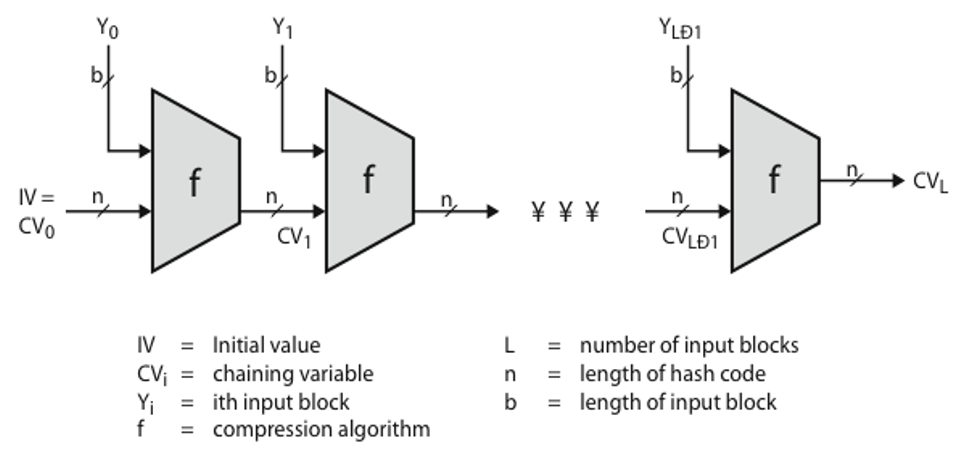
\includegraphics[width=\textwidth]{hash_algo_structure}
		
	\subsection{Digital Signatures}
		\paragraph{} A popular application of message digest or hash functions is digital signatures. Computing a digital signature for a long message is very time-consuming. However, computing a digital signature for a message that is only 128 or 160 bits long can be done quickly. So, instead of digitally signing the message, the message's hash is signed. 
		\paragraph{} To verify the signature, the recipient of the message computes the hash of the message he received. He compares this against the fingerprint that was signed. If they are the same, then (because of the second property above), the message he received is authentic.
		\paragraph{} Should an attacker have manipulated the message, then the fingerprint of the manipulated message will be very different from the fingerprint that has been signed by the sender. The attacker is not able to create a new fingerprint that is signed by the original sender.
	
	\subsection{Integrity Verification}
		\paragraph{} File transmissions over networks such as the Internet may sometimes introduce small errors. To verify whether the received file is identical to the original, the recipient computes the hash of the received file. This hash is then compared to the hash of the original file. That original hash was published on the website or FTP site where the original can be downloaded. It could also be transmitted along with the file.
		
		\paragraph{} This use of hash functions is comparable to the use of checksums or Cyclic Redundancy Check (CRC) functions. However CRC functions typically produce outputs of only 32 bits long. It is easy to find a different input that produces the same 32-bit output.
		
		\paragraph{} In this scenario, tampering with the original file cannot be detected. If that is also desirable, the creator of the original file should not just publish the hash but should digitally sign that hash first. 
		
\section{Algorithm}
	\paragraph{} SHA1 algorithm consists of 6 tasks:
	\begin{enumerate}
		\item  \textbf{Appending Padding Bits:} The original message is "padded" (extended) so that its length (in bits) is congruent to 448, modulo 512. The padding rules are: 
			\begin{itemize}
				\item The original message is always padded with one bit "1" first.
				\item Then zero or more bits "0" are padded to bring the length of the message up to 64 bits fewer than a multiple of 512.					
			\end{itemize}
		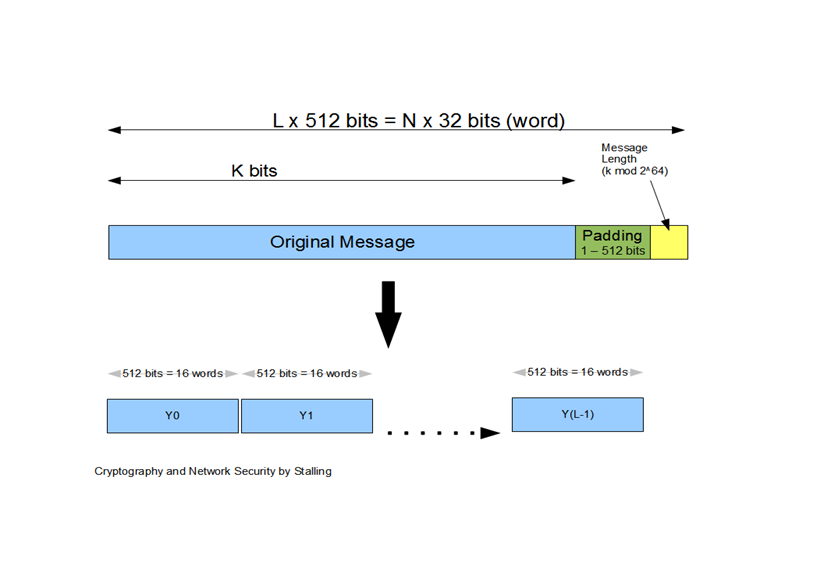
\includegraphics[width=\textwidth]{message_padding}		
			
		\item \textbf{Appending Length:} 64 bits are appended to the end of the padded message to indicate the length of the original message in bytes. The rules of appending length are:
			\begin{itemize}
				\item The length of the original message in bytes is converted to its binary format of 64 bits. If overflow happens, only the low-order 64 bits are used. 
				\item Break the 64-bit length into 2 words (32 bits each). 
				\item The low-order word is appended first and followed by the high-order word. 
			\end{itemize} 
		\item \textbf{Preparing Processing Functions:} SHA1 requires 80 processing functions defined as: \\\\
		\begin{codefont}
			f(t;B,C,D) = (B AND C) OR ((NOT B) AND D)\\        >\qquad ( 0 <= t <= 19)\\ 
			f(t;B,C,D) = B XOR C XOR D\\                       >\qquad (20 <= t <= 39)\\ 
			f(t;B,C,D) = (B AND C) OR (B AND D) OR (C AND D)\\ >\qquad (40 <= t <= 59)\\ 
			f(t;B,C,D) = B XOR C XOR D\\                       >\qquad (60 <= t <= 79)\\ 
		\end{codefont}
        
        \item \textbf{Preparing Processing Constants:} SHA1 requires 80 processing constant words defined as: \\\\
        \begin{codefont}
			K(t) = 0x5A827999         ( 0 <= t <= 19)\\ 
   			K(t) = 0x6ED9EBA1         (20 <= t <= 39)\\ 
   			K(t) = 0x8F1BBCDC         (40 <= t <= 59)\\ 
   			K(t) = 0xCA62C1D6         (60 <= t <= 79)\\ 
		\end{codefont}
        
    	\item \textbf{Initializing Buffers:} SHA1 algorithm requires 5 word buffers with the following initial values:\\\\
        \begin{codefont}
			H0 = 0x67452301\\
   			H1 = 0xEFCDAB89\\
   			H2 = 0x98BADCFE\\
   			H3 = 0x10325476\\
   			H4 = 0xC3D2E1F0\\
		\end{codefont}
        
        \vspace{30px}
        
        \item \textbf{Processing Message in 512-bit Blocks:} This is the main task of SHA1 algorithm, which loops through the padded and appended message in blocks of 512 bits each. For each input block, a number of operations are performed. This task can be described in the following pseudo code slightly modified from the RFC 3174's method 1:\\\\
        
        \item \textbf{Algorithm}
	\lstset{language=Python}
\begin{lstlisting}
For loop on k = 1 to N
	(W(0),W(1),...,W(15)) = M[k] /* Divide M[k] into 16 words */

For t = 16 to 79 do:
	W(t) = (W(t-3) XOR W(t-8) XOR W(t-14) XOR W(t-16)) <<< 1

A = H0, B = H1, C = H2, D = H3, E = H4

For t = 0 to 79 do:
	TEMP = A<<<5 + f(t;B,C,D) + E + W(t) + K(t)
	E = D, D = C, C = B<<<30, B = A, A = TEMP
End of for loop

H0 = H0 + A, H1 = H1 + B, H2 = H2 + C, H3 = H3 + D, H4 = H4 + E
End of for loop

Output: 
H0, H1, H2, H3, H4, H5: Word buffers with final message digest
\end{lstlisting}
\end{enumerate} 


\section{Conclusion}
	\paragraph{} Thus, we have studied and implemented SHA algorithm to obtain digest of given message.
\vspace{20px}
\begin{center}
	\begin{tabular}
		{|c|c|c|c|}\hline
		{\bf Roll No.}		&{\bf Name of Student}		&{\bf Date of Performance}  				&{\bf Date of Submission}  \\ \hline
		{302}	&	{Abhinav Bakshi}& {31/12/2016}		&  {21/01/2016} \\ \hline
	\end{tabular}\\ 
\end{center}


\section{Plagarism Report}
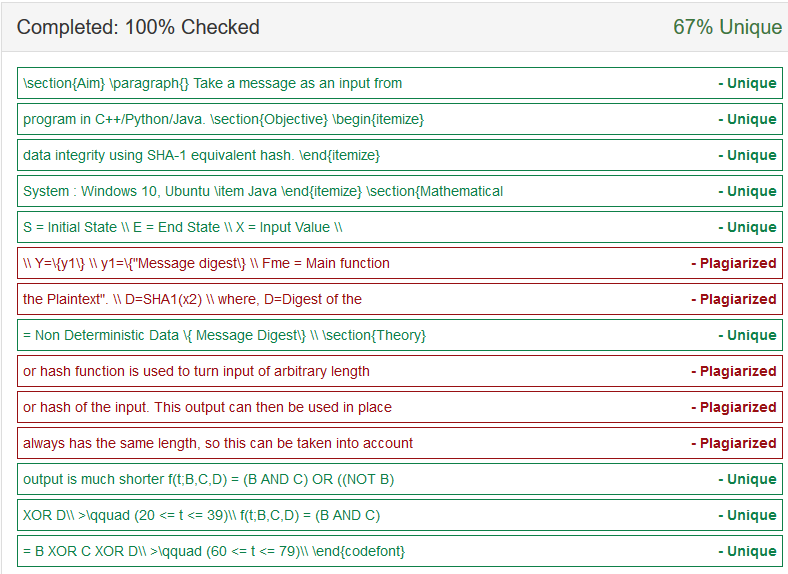
\includegraphics[width=\textwidth]{sha}
\section{Output}
\begin{verbatim}
-------------------------------------------
SHA output

Please enter the message : 
The quick brown fox jumps over the lazy dog


Given Message is : The quick brown fox jumps over the lazy dog
Padding
Converting Message into HexString
Creating word array
Initialization of A,B,C,D,E VALUES
H0:2fd4e1c6
H0:7a2d28fc
H0:ed849ee1
H0:bb76e739
H0:1b93eb12
Output: 2fd4e1c67a2d28fced849ee1bb76e7391b93eb12

Please enter the message : 
The quick brown fox jumps over the lazy cog


Given Message is : The quick brown fox jumps over the lazy cog
Padding
Converting Message into HexString
Creating word array
Initialization of A,B,C,D,E VALUES
H0:de9f2c7f
H0:d25e1b3a
H0:fad3e85a
H0:bd17d9b
H0:100db4b3
Output: de9f2c7fd25e1b3afad3e85a0bd17d9b100db4b3

-------------------------------------------------------------

\end{verbatim}
\end{document}
 

 
